\hypertarget{integrauxe7uxe3o-scada-clp-iot-cloud}{%
\chapter{Integração SCADA + CLP + IoT + Cloud}\label{integrauxe7uxe3o-scada-clp-iot-cloud}}

\section*{Objetivos de Aprendizagem}

Ao final deste capítulo, o leitor será capaz de:

\begin{itemize}
\tightlist
\item
  Desenhar uma arquitetura de referência que integre controlador, supervisão, borda e nuvem.
\item
  Decidir em qual camada cada função deve morar e justificar a escolha.
\item
  Montar a sequência de dados de integrações típicas, do sensor ao painel.
\item
  Reconhecer as falhas de integração mais comuns e o teste que as revela.
\item
  Aplicar a regra que separa supervisão de comando em arquiteturas híbridas.
\end{itemize}

\begin{center}\rule{0.5\linewidth}{0.5pt}\end{center}

\hypertarget{quatro-mundos-um-dado-suxf3}{%
\section{Quatro mundos, um dado só}\label{quatro-mundos-um-dado-suxf3}}

O CLP, o SCADA, o mundo IoT e a nuvem têm requisitos que não se parecem:

\textbf{Tabela 18.1 -- Requisitos que precisam conviver}

\begin{longtable}[]{@{}
  >{\raggedright\arraybackslash}p{(\columnwidth - 6\tabcolsep) * \real{0.2500}}
  >{\raggedright\arraybackslash}p{(\columnwidth - 6\tabcolsep) * \real{0.2500}}
  >{\raggedright\arraybackslash}p{(\columnwidth - 6\tabcolsep) * \real{0.2500}}
  >{\raggedright\arraybackslash}p{(\columnwidth - 6\tabcolsep) * \real{0.2500}}@{}}
\toprule\noalign{}
\begin{minipage}[b]{\linewidth}\raggedright
Camada
\end{minipage} & \begin{minipage}[b]{\linewidth}\raggedright
Precisa de
\end{minipage} & \begin{minipage}[b]{\linewidth}\raggedright
Não tolera
\end{minipage} & \begin{minipage}[b]{\linewidth}\raggedright
Horizonte de tempo
\end{minipage} \\
\midrule\noalign{}
\endhead
\bottomrule\noalign{}
\endlastfoot
CLP & Determinismo e disponibilidade & Depender de rede ou servidor para proteger & Milissegundos \\
SCADA & Estado atual confiável e comando auditável & Valor mentiroso na tela & Décimos de segundo a segundos \\
Borda & Reduzir, normalizar e guardar & Perder dado quando o enlace cai & Segundos a horas \\
Nuvem & Volume, histórico e visão de conjunto & Ser caminho crítico do processo & Minutos a meses \\
\end{longtable}

A integração dá certo quando cada camada faz o que sabe fazer, e não quando uma tenta substituir a
outra. O Capítulo 6 já estabeleceu que IoT/IIoT não substituem SCADA; aqui a discussão é de projeto:
\textbf{onde colocar cada peça}.

\begin{center}
\IfFileExists{../figuras/capitulo-18-m1.pdf}{%
  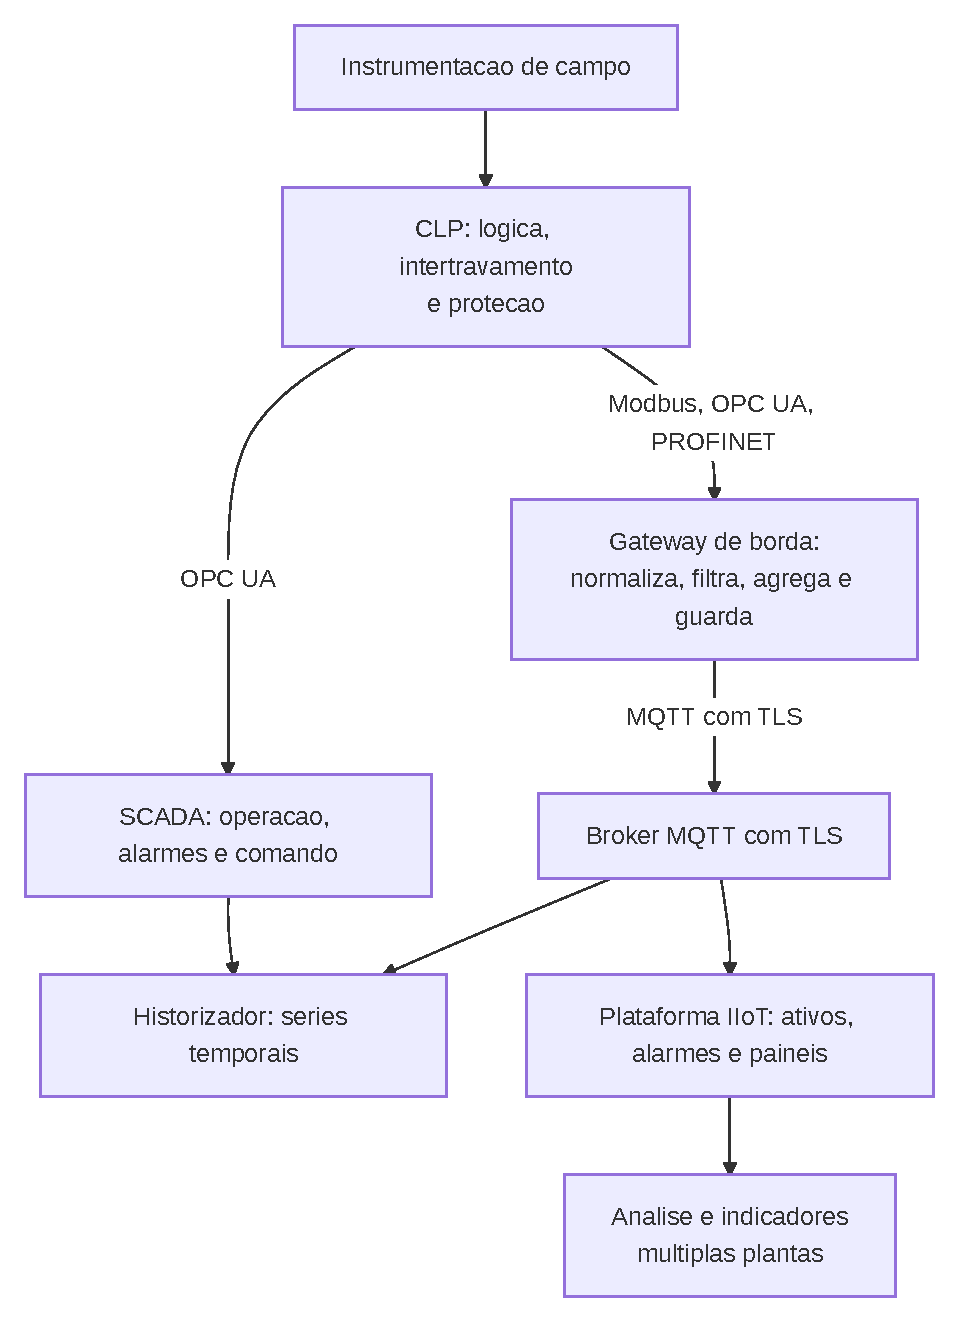
\includegraphics[width=\linewidth,height=0.8\textheight,keepaspectratio]{../figuras/capitulo-18-m1.pdf}%
}{\fbox{\parbox{0.9\linewidth}{\small Diagrama Mermaid ainda não renderizado: capitulo-18-m1. Rode scripts/render-mermaid.sh.}}}
\end{center}

\begin{center}\rule{0.5\linewidth}{0.5pt}\end{center}

\hypertarget{onde-cada-decisuxe3o-deve-morar}{%
\section{Onde cada decisão deve morar}\label{onde-cada-decisuxe3o-deve-morar}}

Esta é a tabela que evita a maior parte dos erros de arquitetura. Ela é curta de propósito.

\textbf{Tabela 18.2 -- Alocação de funções por camada}

\begin{longtable}[]{@{}
  >{\raggedright\arraybackslash}p{(\columnwidth - 4\tabcolsep) * \real{0.3333}}
  >{\raggedright\arraybackslash}p{(\columnwidth - 4\tabcolsep) * \real{0.3333}}
  >{\raggedright\arraybackslash}p{(\columnwidth - 4\tabcolsep) * \real{0.3333}}@{}}
\toprule\noalign{}
\begin{minipage}[b]{\linewidth}\raggedright
Função
\end{minipage} & \begin{minipage}[b]{\linewidth}\raggedright
Camada correta
\end{minipage} & \begin{minipage}[b]{\linewidth}\raggedright
Por quê
\end{minipage} \\
\midrule\noalign{}
\endhead
\bottomrule\noalign{}
\endlastfoot
Intertravamento, proteção, parada de emergência & CLP (ou SIS) & Precisa de determinismo e de independência de rede \\
Sequência de partida e controle regulatório & CLP & Ciclo de varredura adequado e disponibilidade local \\
Supervisão, comando do operador e alarmes de processo & SCADA & Interface, gestão de alarmes e trilha de auditoria (Capítulos 10 e 11) \\
Sincronização de nomes, unidades e faixas & Uma única fonte, aplicada às demais & Evita o mesmo dado com dois significados \\
Redução, agregação e \emph{store and forward} & Borda & É onde o dado é volumoso e o enlace é caro (Capítulo 17) \\
Histórico de alta resolução & Historizador junto ao processo & Consulta rápida e resolução preservada (Capítulo 16) \\
Histórico longo, indicadores e análise entre plantas & Nuvem & Volume, retenção e visão consolidada \\
Detecção de anomalia em série longa e modelos & Nuvem ou planta & Exige histórico consolidado (Capítulo 20) \\
\end{longtable}

\textbf{A regra que não se negocia:} o \textbf{comando} do processo nasce no SCADA ou na IHM local, por
protocolo autenticado, com trilha de auditoria. A nuvem \textbf{observa}. Quando o cliente pede ``quero
ligar a bomba pelo celular'', a resposta de engenharia é: você pode, se o caminho for autenticado,
com autorização por papel, com confirmação de estado de volta e com registro de quem comandou --- e
mesmo assim só para comandos que não afetem segurança.

\begin{figure}
\centering
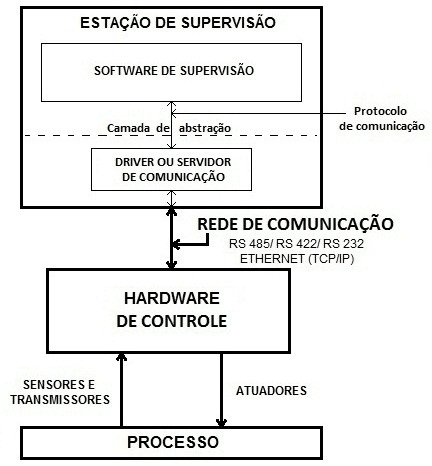
\includegraphics{../figuras/cap18-camada-abstracao.png}
\caption[Figura 18.1 -- Camada de abstração: onde o software de supervisão se separa do hardware de controle]{Figura 18.1 -- Camada de abstração: onde o software de supervisão se separa do hardware de controle. \textbf{Fonte:} \emph{Livro SCADA --- versão para análise}, p.~24 (Machado, Pontes e Vianna, reproduzida com crédito).}
\end{figure}

A figura mostra o conceito que sustenta toda a integração: a \textbf{camada de abstração} permite
implementar a IHM sem conhecer a tecnologia do hardware de controle, e o \textbf{driver} é a peça que
pode ser trocada sem reescrever a aplicação. É por isso que o servidor de comunicação pode agregar
mais de um driver, para hardware e interfaces diferentes, sem que o software de supervisão precise
saber como cada um funciona.

\begin{center}\rule{0.5\linewidth}{0.5pt}\end{center}

\hypertarget{a-sequuxeancia-de-dados-passo-a-passo}{%
\section{A sequência de dados, passo a passo}\label{a-sequuxeancia-de-dados-passo-a-passo}}

Integração se aprende seguindo o dado. Os cinco arranjos abaixo são progressivos e cada um acrescenta
uma peça; todos são usados em plantas reais.

\hypertarget{vuxe1lvula-solenoide-comandada-por-clp}{%
\subsection{Válvula solenoide comandada por CLP}\label{vuxe1lvula-solenoide-comandada-por-clp}}

\textbf{Sequência:} o operador aciona o botão na IHM \ensuremath{\rightarrow} o SCADA escreve \passthrough{\lstinline!1!} no tag de comando \ensuremath{\rightarrow} o driver
grava na memória imagem do CLP \ensuremath{\rightarrow} a lógica energiza a saída \ensuremath{\rightarrow} a solenoide abre \ensuremath{\rightarrow} o sensor de fim de
curso confirma \ensuremath{\rightarrow} o CLP atualiza a entrada \ensuremath{\rightarrow} o driver lê \ensuremath{\rightarrow} o tag de estado muda \ensuremath{\rightarrow} a IHM anima o
objeto.

\textbf{Configuração mínima:} dois tags (comando e estado), faixa morta zero no estado, tempo de retorno
esperado.

\textbf{O que observar no resultado:} o atraso entre comandar e ver o estado; se a confirmação não chega
no tempo esperado, deve existir alarme de falha de atuação --- e não um botão que ``não fez nada''.

\textbf{Limitação:} o comando pelo supervisório não é proteção. Se a válvula precisa fechar por segurança,
quem fecha é o intertravamento, não a IHM.

\hypertarget{clp-scada}{%
\subsection{\texorpdfstring{CLP \ensuremath{\rightarrow} SCADA}{CLP  SCADA}}\label{clp-scada}}

\textbf{Sequência:} leitura da memória do CLP pelo driver \ensuremath{\rightarrow} escalonamento para unidade de engenharia \ensuremath{\rightarrow}
validação de faixa \ensuremath{\rightarrow} avaliação de alarme \ensuremath{\rightarrow} atualização do objeto na tela \ensuremath{\rightarrow} gravação no historizador.

\textbf{Configuração mínima:} classe de varredura por grupo de tags, faixa e unidade no cadastro, limites
de alarme documentados, tendência real com janela dimensionada.

\textbf{O que observar:} a coerência entre o valor exibido e o valor lido localmente no CLP, com o mesmo
instrumento e no mesmo instante.

\textbf{Limitação:} o SCADA é não determinístico --- o atraso da tela não é erro, mas precisa ser conhecido
(Capítulo 15).

\hypertarget{clp-mqtt-plataforma-iiot}{%
\subsection{\texorpdfstring{CLP \ensuremath{\rightarrow} MQTT \ensuremath{\rightarrow} plataforma IIoT}{CLP  MQTT  plataforma IIoT}}\label{clp-mqtt-plataforma-iiot}}

\textbf{Sequência:} a função de cliente MQTT no CLP ou no gateway publica no tópico de telemetria com o
identificador do dispositivo \ensuremath{\rightarrow} a plataforma recebe, registra a telemetria e dispara a cadeia de
regras \ensuremath{\rightarrow} a regra cria ou limpa alarme \ensuremath{\rightarrow} o painel é atualizado.

\textbf{Configuração mínima:} identificador do dispositivo e credencial por dispositivo, estrutura de
tópico, formato do \emph{payload} e carimbo de tempo, além da regra que distingue alarme de registro.

\textbf{O que observar:} o tempo entre a mudança no processo e a atualização do painel; o que acontece
com um valor fora da faixa no motor de alarme.

\textbf{Limitação:} a plataforma não executa controle. Ela observa, registra e notifica (Capítulo 12).

\begin{center}
\IfFileExists{../figuras/capitulo-18-m2.pdf}{%
  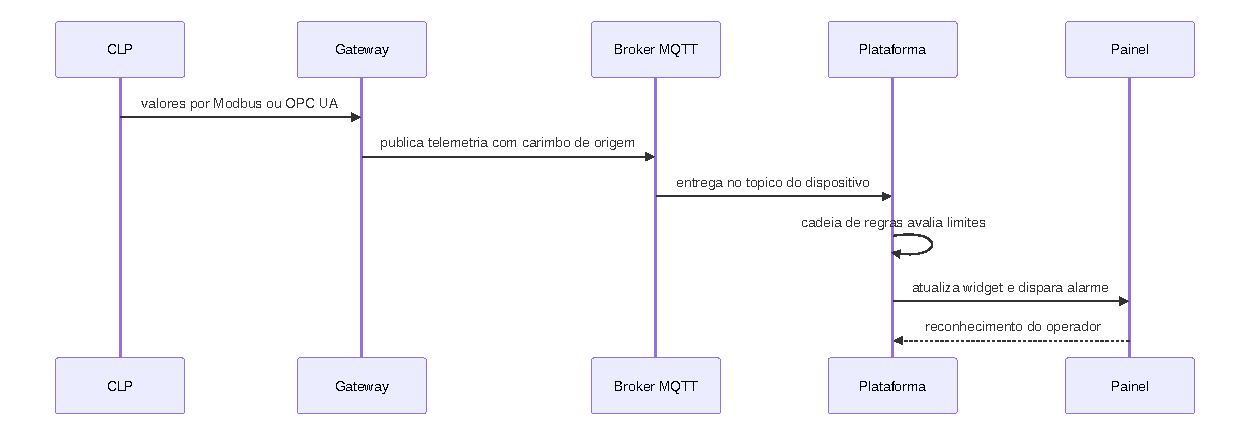
\includegraphics[width=\linewidth,height=0.8\textheight,keepaspectratio]{../figuras/capitulo-18-m2.pdf}%
}{\fbox{\parbox{0.9\linewidth}{\small Diagrama Mermaid ainda não renderizado: capitulo-18-m2. Rode scripts/render-mermaid.sh.}}}
\end{center}

\hypertarget{sensor-node-red-mqtt-plataforma}{%
\subsection{\texorpdfstring{Sensor \ensuremath{\rightarrow} Node-RED \ensuremath{\rightarrow} MQTT \ensuremath{\rightarrow} plataforma}{Sensor  Node-RED  MQTT  plataforma}}\label{sensor-node-red-mqtt-plataforma}}

\textbf{Sequência:} Node-RED lê a fonte (Modbus, serial, HTTP ou simulador) \ensuremath{\rightarrow} normaliza nome e unidade \ensuremath{\rightarrow}
injeta o carimbo de tempo \ensuremath{\rightarrow} publica em MQTT \ensuremath{\rightarrow} a plataforma persiste e apresenta.

\textbf{Configuração mínima:} nó de leitura com \emph{timeout}, tratamento de erro explícito, injeção de
carimbo de tempo e retenção de última mensagem desativada para dado temporal.

\textbf{O que observar:} o comportamento com a fonte fora do ar --- o fluxo precisa \textbf{não publicar} valor
antigo como se fosse atual.

\textbf{Limitação:} Node-RED é excelente para prototipar e mediar, e não é ambiente de controle nem de
garantia temporal (Capítulo 7).

\hypertarget{scada-historiador-dashboard}{%
\subsection{SCADA + historiador + dashboard}\label{scada-historiador-dashboard}}

\textbf{Sequência:} o SCADA coleta e disponibiliza por OPC UA \ensuremath{\rightarrow} o historiador assina as variáveis com
intervalo de amostragem e faixa morta definidos \ensuremath{\rightarrow} o dashboard consulta o histórico por período e
agregação.

\textbf{Configuração mínima:} o que é gravado, com que resolução e por quanto tempo (Capítulo 16); a
consulta do painel com agregação explícita.

\textbf{O que observar:} a diferença entre o valor lido na tela do SCADA e o ponto mais próximo no
histórico --- se for grande, a faixa morta ou o filtro estão escondendo o transitório.

\textbf{Limitação:} painel não é sistema de operação. Ninguém deve comandar o processo por dashboard.

\begin{caixafigura}

\textbf{{[}Figura 18.2 -- Caminho completo do dado, de ponta a ponta{]}}
\emph{Diagrama em faixas horizontais, no estilo de arquitetura de referência: no alto a instrumentação; abaixo o CLP com a lógica e o intertravamento destacados; em seguida a borda com as duas faces e a fila local; depois, em paralelo, o SCADA com estação de operação e o historizador; por último o broker, a plataforma e a análise. Sobre as setas, anotar protocolo e sentido; nas laterais, marcar com cadeado os trechos cifrados e anotar o carimbo de tempo em cada troca.}

\end{caixafigura}

\begin{center}\rule{0.5\linewidth}{0.5pt}\end{center}

\hypertarget{onde-a-integrauxe7uxe3o-costuma-quebrar}{%
\section{Onde a integração costuma quebrar}\label{onde-a-integrauxe7uxe3o-costuma-quebrar}}

Nenhuma dessas falhas é de protocolo. Todas são de projeto, e todas aparecem no mesmo lugar: no
número que está errado na tela de alguém.

\textbf{Tabela 18.3 -- Falhas típicas e sua origem}

\begin{longtable}[]{@{}
  >{\raggedright\arraybackslash}p{(\columnwidth - 4\tabcolsep) * \real{0.3333}}
  >{\raggedright\arraybackslash}p{(\columnwidth - 4\tabcolsep) * \real{0.3333}}
  >{\raggedright\arraybackslash}p{(\columnwidth - 4\tabcolsep) * \real{0.3333}}@{}}
\toprule\noalign{}
\begin{minipage}[b]{\linewidth}\raggedright
Sintoma
\end{minipage} & \begin{minipage}[b]{\linewidth}\raggedright
Causa provável
\end{minipage} & \begin{minipage}[b]{\linewidth}\raggedright
Prevenção
\end{minipage} \\
\midrule\noalign{}
\endhead
\bottomrule\noalign{}
\endlastfoot
O mesmo ativo tem três nomes diferentes & Nenhuma fonte única de nomes & Dicionário de dados único, aplicado às três camadas \\
Valor plausível e errado & Faixa ou unidade divergente entre CLP, cadastro e plataforma & Um cadastro por variável, revisado na partida \\
Sensor com defeito aparece como zero & Qualidade do dado descartada no caminho & Propagar \passthrough{\lstinline!StatusCode!} até a tela (Capítulos 14 e 15) \\
Ordem dos eventos não fecha & Carimbo atribuído em pontos diferentes da cadeia & Carimbo na origem e relógios sincronizados \\
Buraco no histórico em dia de problema & Ausência de fila local ou de \emph{store and forward} & Fila dimensionada e testada com o enlace desligado \\
Alarmes duplicados no SCADA e na plataforma & Mesma condição avaliada em duas camadas, com limites diferentes & Um lugar avalia, o outro registra \\
Consumo de dados estourou a franquia & Publicação periódica de tudo & Publicação por exceção com \emph{refresh} (Capítulo 17) \\
\end{longtable}

\begin{center}\rule{0.5\linewidth}{0.5pt}\end{center}

\hypertarget{como-provar-que-a-integrauxe7uxe3o-funciona}{%
\section{Como provar que a integração funciona}\label{como-provar-que-a-integrauxe7uxe3o-funciona}}

Integração não se valida lendo configuração; valida-se \textbf{injetando perturbação}. O roteiro mínimo:

\begin{enumerate}
\def\labelenumi{\arabic{enumi}.}
\tightlist
\item
  \textbf{Valor conhecido.} Injete um valor de teste no instrumento ou simule a fonte e siga o número por
  todas as camadas até o painel, conferindo unidade, faixa e casas decimais.
\item
  \textbf{Corte de enlace.} Desligue a comunicação por tempo significativo e verifique se o dado volta
  completo e com o carimbo correto.
\item
  \textbf{Reinício de nó.} Reinicie o gateway, o broker e a estação, um por vez, e observe o que cada
  reinício faz com a série e com os alarmes.
\item
  \textbf{Valor fora de faixa.} Envie um valor fisicamente impossível e verifique se ele é rejeitado com
  qualidade ruim em vez de alarmar o operador.
\item
  \textbf{Mudança de horário.} Desloque o relógio de um nó e verifique se a divergência é detectada.
\item
  \textbf{Desligamento da nuvem.} Deixe a plataforma fora do ar e confirme que o SCADA e o CLP continuam
  operando normalmente.
\end{enumerate}

\begin{caixadica}

\textbf{Dica:} transforme esses seis testes em um procedimento de aceitação com registro de resultado
e data. Um sistema integrado sem esse registro é um sistema que ninguém sabe se está funcionando ---
só se sabe que ainda não falhou de forma visível.
\textbf{{[}Figura 18.3 -- Registro do teste de corte de enlace{]}}
\emph{Captura de uma tabela de procedimento de aceitação preenchida: colunas de item testado, condição imposta (enlace desligado por 2 h, entre 09h00 e 11h00), resultado esperado, resultado observado e responsável. Duas linhas em destaque: ``dado recuperado com carimbo de origem'' e ``nenhum registro gravado com horário de reconexão''. Ao lado, o gráfico da série temporal mostrando o trecho sem recepção e o preenchimento posterior da curva no intervalo correto.}
---

\end{caixadica}

\hypertarget{estudo-de-caso-a-integrauxe7uxe3o-que-duplicou-os-alarmes}{%
\section{\texorpdfstring{Estudo de Caso --- A integração que duplicou os alarmes}{Estudo de Caso  A integração que duplicou os alarmes}}\label{estudo-de-caso-a-integrauxe7uxe3o-que-duplicou-os-alarmes}}

\textbf{Cenário.} Uma indústria de alimentos integrou o SCADA existente a uma plataforma IIoT para dar
visão de indicadores à gestão. Seis meses depois, a plataforma foi liberada também para a supervisão
móvel dos coordenadores de turno, com notificação por mensagem.

\textbf{Diagnóstico.} No primeiro mês de uso, a operação reclamou de ``alarme repetido no celular sem nada
de errado na tela do SCADA''. A análise mostrou três problemas sobrepostos:

\begin{enumerate}
\def\labelenumi{\arabic{enumi}.}
\tightlist
\item
  A plataforma avaliava limites próprios, digitados na configuração dos dispositivos, diferentes dos
  limites do SCADA --- o alarme de temperatura alta da plataforma disparava 2 \ensuremath{^\circ}C antes.
\item
  Não havia faixa morta na plataforma, e a variável oscilava em torno do limite: o celular recebia
  dezenas de mensagens por turno.
\item
  Os alarmes da plataforma não eram reconhecidos por ninguém: o operador reconhecia no SCADA, e a
  plataforma continuava notificando.
\end{enumerate}

\textbf{Decisão de engenharia.}

\begin{longtable}[]{@{}
  >{\raggedright\arraybackslash}p{(\columnwidth - 2\tabcolsep) * \real{0.5000}}
  >{\raggedright\arraybackslash}p{(\columnwidth - 2\tabcolsep) * \real{0.5000}}@{}}
\toprule\noalign{}
\begin{minipage}[b]{\linewidth}\raggedright
Problema
\end{minipage} & \begin{minipage}[b]{\linewidth}\raggedright
Medida
\end{minipage} \\
\midrule\noalign{}
\endhead
\bottomrule\noalign{}
\endlastfoot
Limites divergentes & Limites passaram a ser atributos de configuração, geridos em um só lugar e distribuídos para SCADA e plataforma \\
Alarme espúrio & Faixa morta e atraso de confirmação configurados na plataforma, iguais aos do SCADA \\
Reconhecimento sem efeito & Reconhecimento unificado: quem reconhece no SCADA encerra a notificação na plataforma \\
Papel indefinido & Notificação móvel restrita a alarmes de prioridade alta e de equipamento, com registro de quem recebeu \\
\end{longtable}

\textbf{Resultado.} As mensagens por turno caíram de algumas dezenas para menos de cinco, e voltaram a ser
lidas. O ganho não veio de tecnologia nova: veio de decidir quem avalia o quê e de um único lugar
para os limites.

\textbf{Limitações do arranjo.} O reconhecimento unificado exige um identificador comum de alarme nas duas
camadas e não funciona com plataformas que geram o seu próprio identificador sem correlação. E a
decisão de restringir a notificação por prioridade deixou a plataforma cega para alarmes de processo
de prioridade média --- o que foi aceito como decisão de projeto, não como efeito colateral.

\begin{center}\rule{0.5\linewidth}{0.5pt}\end{center}

\hypertarget{resumo}{%
\section{Resumo}\label{resumo}}

\begin{itemize}
\tightlist
\item
  Cada camada tem um \textbf{horizonte de tempo} próprio: milissegundos no CLP, segundos no SCADA, horas na borda, meses na nuvem.
\item
  A alocação de funções é o que define o sucesso da integração, e não o protocolo escolhido.
\item
  \textbf{Comando} nasce no SCADA ou na IHM local, com autenticação e trilha; a nuvem observa.
\item
  Integração se aprende seguindo o dado: cada arranjo (CLP \ensuremath{\rightarrow} SCADA, CLP \ensuremath{\rightarrow} MQTT \ensuremath{\rightarrow} plataforma, sensor \ensuremath{\rightarrow} Node-RED \ensuremath{\rightarrow} plataforma, SCADA + historian + dashboard) acrescenta uma peça.
\item
  As falhas de integração são de \textbf{modelagem}: nomes divergentes, faixa errada, qualidade descartada, carimbo no lugar errado.
\item
  O mesmo dado não deve ser avaliado em duas camadas com limites diferentes: \textbf{um lugar avalia, o outro registra}.
\item
  Integração se valida \textbf{injetando perturbação} --- corte de enlace, reinício, valor fora de faixa, desligamento da nuvem.
\item
  Nenhuma dessas arquiteturas substitui CLP e SCADA no controle, na proteção e na segurança funcional.
\end{itemize}

\hypertarget{questuxf5es-de-revisuxe3o}{%
\section{Questões de Revisão}\label{questuxf5es-de-revisuxe3o}}

\begin{enumerate}
\def\labelenumi{\arabic{enumi}.}
\tightlist
\item
  Explique por que o determinismo do CLP e a imprevisibilidade da nuvem exigem uma arquitetura em camadas, e não um único sistema.
\item
  Preencha a alocação de funções para um projeto de sua escolha, indicando em que camada ficam intertravamento, alarme de processo, agregação e análise preditiva.
\item
  Descreva a sequência completa de dados de um comando de abertura de válvula pela IHM, identificando onde pode haver atraso.
\item
  Por que a nuvem não deve comandar o processo? Cite duas exceções aceitáveis e as condições que as tornam seguras.
\item
  Um operador reclama que o valor de vazão no dashboard é 5 \% menor que na tela do SCADA. Liste quatro causas possíveis e como verificar cada uma.
\item
  Descreva o que deve acontecer com a série temporal quando o enlace é desligado por quatro horas e restabelecido.
\item
  Explique por que a mesma condição avaliada no SCADA e na plataforma gera alarme duplicado, e proponha a correção.
\item
  Monte um roteiro de aceitação de integração com seis testes de perturbação e o resultado esperado em cada um.
\item
  Uma planta quer publicar 800 variáveis por MQTT a cada 5 s em enlace 4G com franquia de 20 GB mensais. Estime o volume, critique a proposta e apresente uma arquitetura alternativa.
\end{enumerate}

\hypertarget{referuxeancias}{%
\section{Referências}\label{referuxeancias}}

\begin{itemize}
\tightlist
\item
  MACHADO, R.; PONTES, W.; VIANNA, W. \textbf{Livro SCADA --- versão para análise}. Material didático do curso (arquitetura básica, servidor de comunicação, camada de abstração e sistema web server). Figura reproduzida com crédito.
\item
  VIANNA, W. S. \textbf{Sistema SCADA Supervisório}. IFF, 2008 (arquiteturas típicas de sistemas SCADA, com CLP, fieldbus, controladores dedicados e controle digital direto; tecnologias web).
\item
  INTERNATIONAL SOCIETY OF AUTOMATION. \textbf{ISA-95 / IEC 62264 --- Enterprise-control system integration} (integração entre níveis de automação e de gestão; verificar edição vigente).
\item
  OPC FOUNDATION. \textbf{OPC Unified Architecture} --- cliente-servidor e PubSub aplicados à integração entre equipamento, supervisão e nuvem. Disponível em: opcfoundation.org. Consulta: 2026.
\item
  ECLIPSE FOUNDATION. \textbf{Sparkplug Specification 3.0} --- convenção de tópicos e estados de sessão para integração IIoT. Disponível em: \url{eclipse.org/tahu}. Consulta: 2026.
\item
  THINGSBOARD. \textbf{Documentação oficial} --- telemetria, atributos, motor de regras, alarmes e RPC. Disponível em: \url{thingsboard.io/docs}. Consulta: 2026.
\item
  GRAFANA LABS. \textbf{Grafana Documentation} --- consulta a séries temporais e painéis de supervisão. Disponível em: \url{grafana.com/docs}. Consulta: 2026.
\end{itemize}
